% sample.tex
\documentclass[pdf,swa,slideBW,nocolorBG,nototal]{prosper}
%\usepackage{ngerman}
\usepackage{graphicx}
\usepackage{wrapfig, rotating}
\usepackage[T1]{fontenc}

\title{Tracing Object Lifetime}
\author{Christoph Neijenhuis, Tobias Mohr, Tim Felgentreff}
%\email{\{christoph.neijenhuis, tobias.mohr, fim.felgentreff\}@student.hpi.uni-potsdam.de}
\institution{
        Agile Software Development \\
        Hasso-Plattner-Institut \\
        Universit�t Potsdam\\
        SS 2011
}
\foot{Agile Software Development 2011 | Felgentreff, Mohr, Neijenhuis | \today }

\begin{document}

\maketitle

\begin{slide}{Demo}
  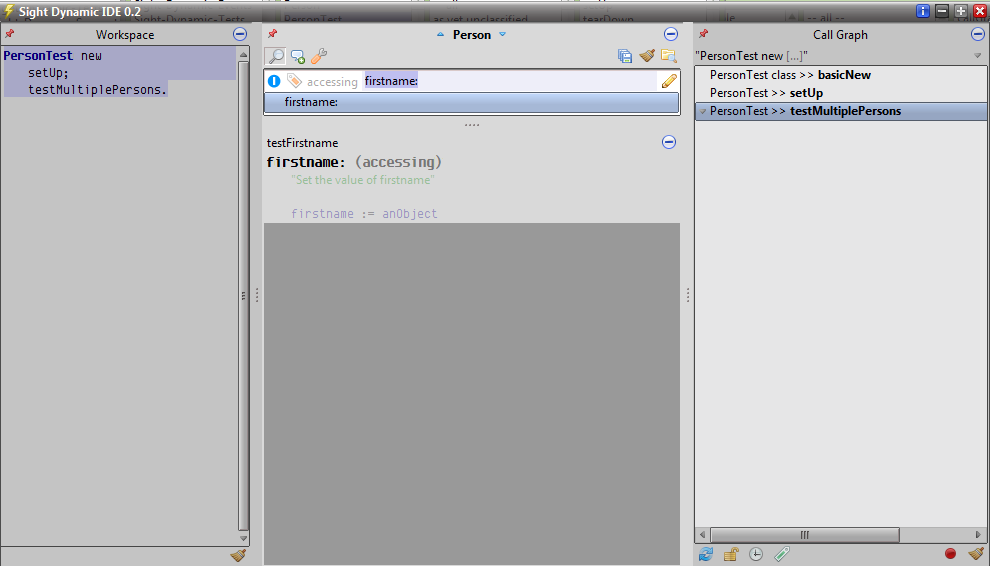
\includegraphics[width=\linewidth]{pics/sdide_intro}
\end{slide}

\begin{slide}{Sight Dynamic IDE}
  \begin{itemize}
  \item A new development tool for Squeak
  \item Column layout to open and combine tools
  \item Easily extended with new tools
    \begin{itemize}
    \item So we did \ldots
    \end{itemize}
  \end{itemize}
\end{slide}

\overlays{2}{%
\begin{slide}{Sight Dynamic Call Graph Tools}
  \begin{itemize}
  \item During its lifetime an object is \ldots
    \begin{itemize}
    \item created from a class,
    \item referenced in different contexts,
    \item passed as parameters,
    \item called upon,
    \item and modified.
    \end{itemize}
  \end{itemize}
  \fromSlide{2}{%
  \begin{itemize}
    \item The call graph tracer is a way to ask questions
    \begin{itemize}
    \item Where did this object come from?
    \item Who calls it and when?
    \item What kind of parameters are passed to the calls?
    \item Where and how is the object modified?
    \item Where does it travel through the calls?
    \end{itemize}
  \end{itemize}}
\end{slide}}

\begin{slide}{Agenda}
  \begin{itemize}
  \item Infrastructure
  \item Planning
  \item User stories
  \item Tests
  \end{itemize}
\end{slide}

\begin{slide}{Infrastructure}
  \parbox[t]{0.6\textwidth}{%
    \vspace*{1.7cm}
    \hspace*{5.5cm}
    \begin{rotate}{0}
      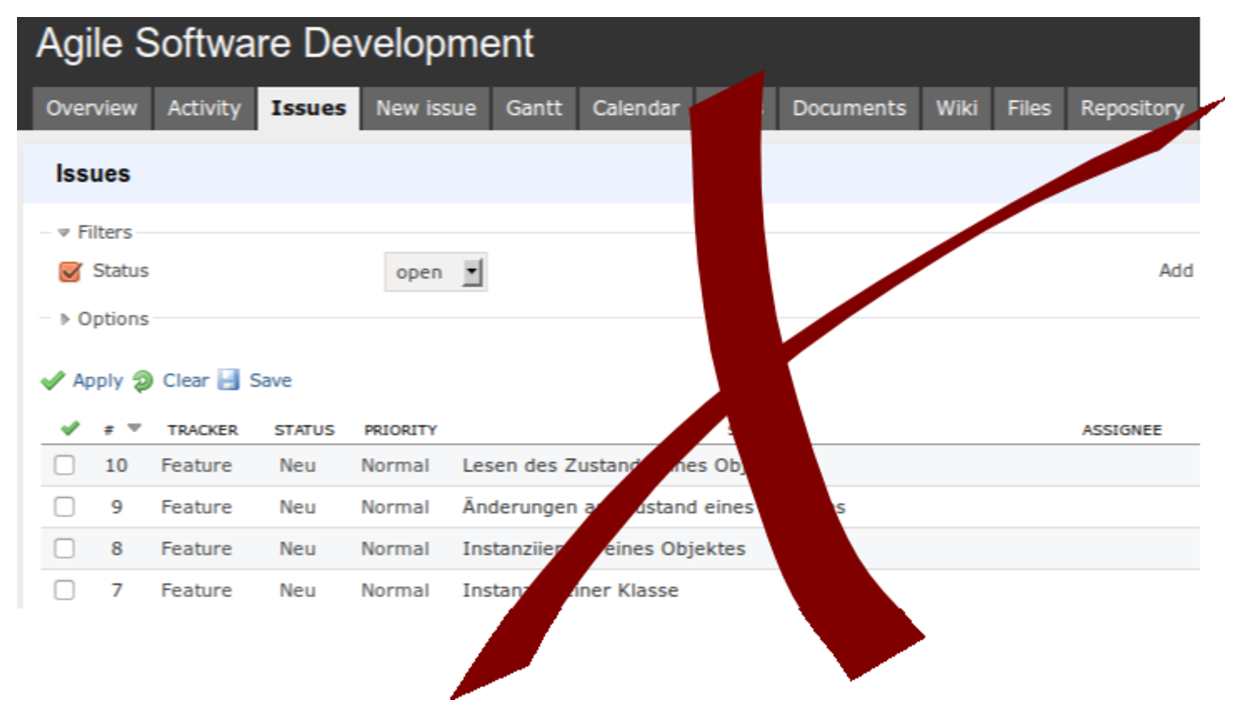
\includegraphics[width=0.6\linewidth]{pics/redmine}
    \end{rotate}}
  \parbox[t]{0.6\textwidth}{%
    \vspace*{4.8cm}
    \hspace*{5.8cm}
    \begin{rotate}{0}
      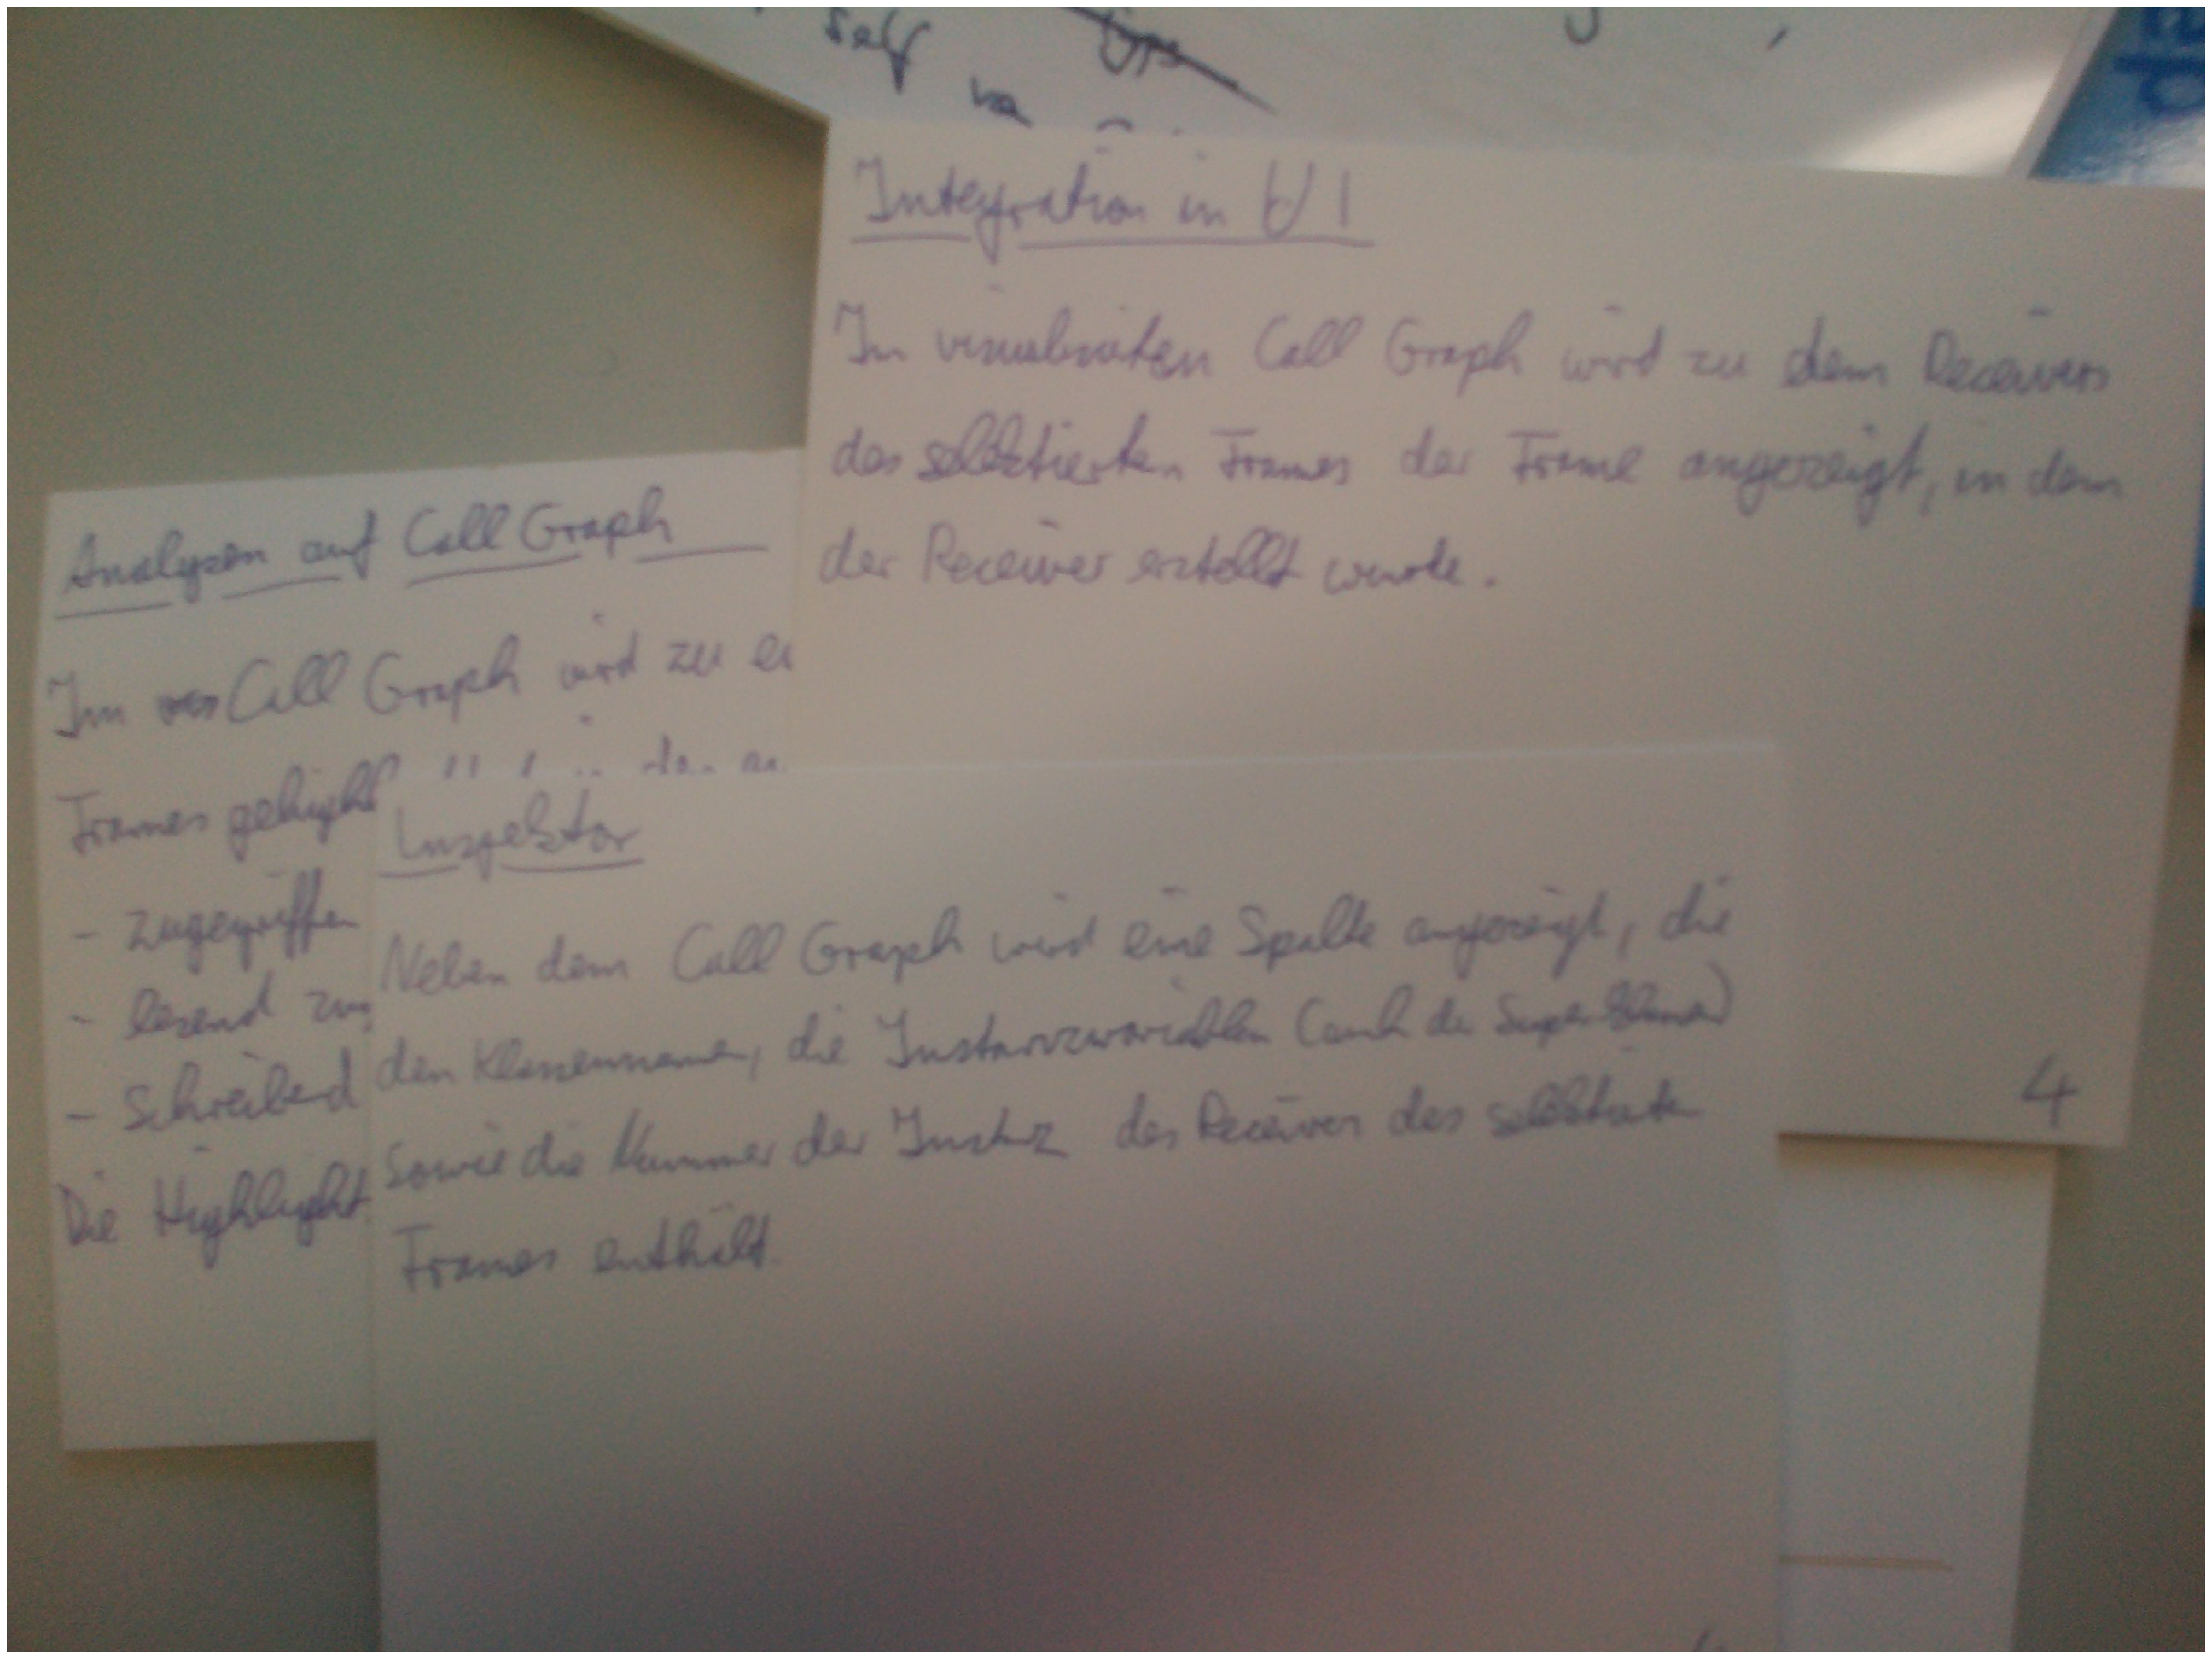
\includegraphics[width=0.9\linewidth]{pics/user_stories}
    \end{rotate}}
  \vspace*{-8cm}
  \begin{itemize}
  \item {\it Full-blown ticket system} ~\\~\\~\\~\\
  \item {\bf Management with ``offline'' story cards}
    \begin{itemize}
    \item Created during bi-weekly\\meetings
    \item Chosen, estimated,\\confirmed and committed to\\with the customer
    \end{itemize}
  \end{itemize}
\end{slide}

\begin{slide}{Planning}
  \begin{itemize}
  \item Bi-weekly meetings
  \item Meetings grew shorter with time
  \item Our understanding of the customer's problem grew
  \item We tried to ``make it our project''
    \begin{itemize}
    \item Actively taking an interest simplifies communication
    \item The customer is constrained by different projects,
      providing stories of our own evokes positive reactions
    \end{itemize}
  \end{itemize}
\end{slide}

\begin{slide}{Planning}
  \begin{itemize}
  \item Building a backlog is important
    \begin{itemize}
      \item \ldots to have something to discuss with the customer
      \item \ldots to have a choice of tasks for the next sprint
      \item \ldots to have a better idea of what's to come
    \end{itemize}
  \item Having more ideas to discuss sharpens the picture of where
    we are headed
  \item With stories to choose from, the customer is forced to exclude
    some ideas
    \begin{itemize}
    \item \ldots something the customer didn't easily admit to
    \end{itemize}
  \item The customer wants solutions, not better descriptions or more plans
  \end{itemize}
\end{slide}

\begin{slide}{User Stories}
  \parbox[t]{0.6\textwidth}{%
    \vspace*{3.5cm}
    \hspace*{5cm}
    \begin{rotate}{353}
      
\includegraphics[width=\linewidth]{pics/user_story}
    \end{rotate}}
  \vspace*{-2.5cm}
  \begin{itemize}
  \item Written during customer\\meetings or by ourselves
  \item Titled for quick reference\\(easier to remember than numbers)
  \item Sometimes accompanied with sketches
  \end{itemize}
\end{slide}

\overlays{4}{%
\begin{slide}{Tests - First Contact}
  \parbox[t]{0.6\textwidth}{%
    \vspace*{2.5cm}
    \hspace*{7cm}
    \begin{rotate}{353}
      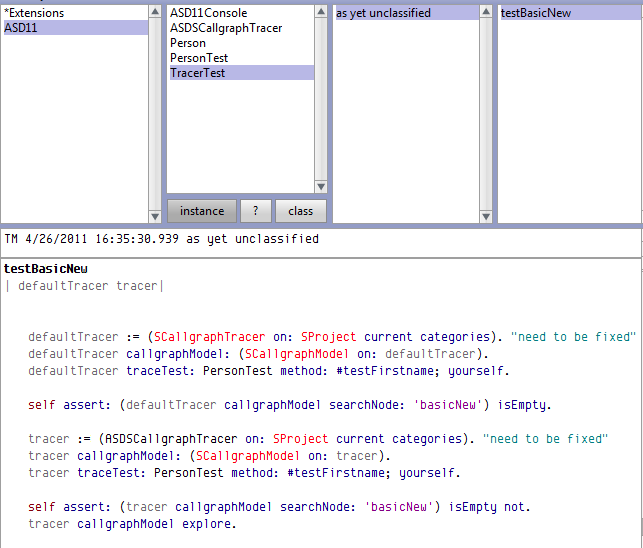
\includegraphics[width=0.7\linewidth]{pics/workspace_test}
    \end{rotate}}
  \vspace*{-2cm}
  \begin{itemize}
  \item Hard to ``test-ahead'' at first
  \item Tests were developed in parallel to the implementation
    \fromSlide{2}{%
      \begin{itemize}
      \item As a quicker workspace
      \item To run examples quickly
      \fromSlide{3}{%
      \item \ldots, but not to test user stories}
    \end{itemize}}
  \fromSlide{4}{%
  \item Code-first $\Rightarrow$ hard to test code
  \item Our first test were hard to read}
  \end{itemize}
\end{slide}}

\begin{slide}{Tests - Ensuring Traceability}
  \parbox[t]{0.6\textwidth}{%
    \vspace*{2.5cm}
    \hspace*{3cm}
    \begin{rotate}{353}
      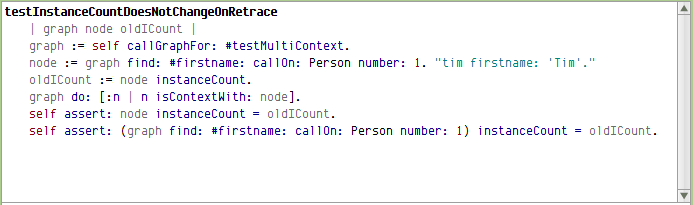
\includegraphics[width=1.5\linewidth]{pics/good_test}
    \end{rotate}}
  % \vspace*{1.5cm}
  \begin{itemize}
  \item Forcing ourselves to write {\sc X} tests for each story card
    \begin{itemize}
    \item More readable tests
    \item More consistent {\sc API}
    \item Better estimates
    \end{itemize}
  \end{itemize}
\end{slide}

\begin{slide}{Tests Have to Run}
  \centering
  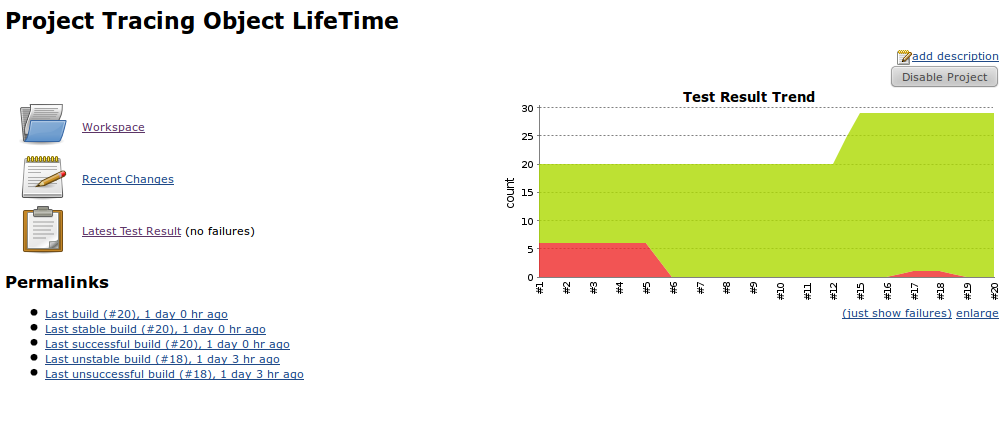
\includegraphics[width=\linewidth]{pics/ci}
  \begin{itemize}
  \item Continuous Integration
  \end{itemize}
\end{slide}

\overlays{3}{%
\begin{slide}{Conclusions}
  \begin{itemize}
  \item The customer's and the developer's visions need to be
    substantiated before they can be discussed
  \fromSlide{2}{%
  \item Steady progress was be achieved by
    \begin{itemize}
    \item \ldots building a backlog
    \item \ldots and taking an interest
    \end{itemize}}
  \fromSlide{3}{%
  \item We've gotten good estimating story times
  \item We still tend to forget non-story tasks, if we don't write
    them down
  \item ``Test first'' works very well, now we have a ``testable'' API
    --- just needed to sit down and do-it\texttrademark}
  \end{itemize}
\end{slide}}

\begin{slide}{}
  \nocite{*}
  \bibliographystyle{splncs}
  {\small \bibliography{swt.bib}}
\end{slide}

\end{document}
